\chapter{Aanleiding voor het project}
%Nu duidelijk is hoe het bedrijf of de organisatie in elkaar steekt vertel je in dit hoofdstuk wat de achtergrond is van het project dat je gaat doen. Waarom is dit project op de agenda terecht gekomen? Wat is de reden dat het bedrijf juist nu dit project wil laten uitvoeren (en niet een ander project)?
De opdrachtever, Allianz Group, verzekerd panden voor miljoenen. Dit type van verzekeringen worden in de praktijk gedeeld met meerdere verzekeraars, om zo het risico te verspreiden. Het probleem waar de opdrachtgever heeft is dat het claimproces erg veel tijd kost voordat deze wordt uitgekeerd naar de klant. Dit komt doordat verschillende instanties met handmatig bedrijfsprocessen een claim eerst moeten valideren en vervolgens gezamenlijk uitvoeren. Hierdoor kan een claim dus vaak meer dan 3 maanden duren na aanvraag voordat deze werkelijk wordt uitbetaald.\par
Om dit probleem op te lossen heeft Allianz opdracht uitgevoerd bij Headforward om dit huidige proces te automatiseren met de laatste technologieën. Deze opdracht dient als afstudeeropdracht die ik tijdens mijn afstudeerstage als project ga uitvoeren. Hierdoor worden de tijdrovende huidige bedrijfsprocessen vervangen en verdwijnt ook de makelaar in het proces. Uiteindelijk bereikt het bedrijf een snellere claim tijd, waardoor de klant meer tevreden is en het minder geld kost.


(figuur \ref{fig:allianz-blockchain}})

\begin{figure}[h!]
    \begin{center}
        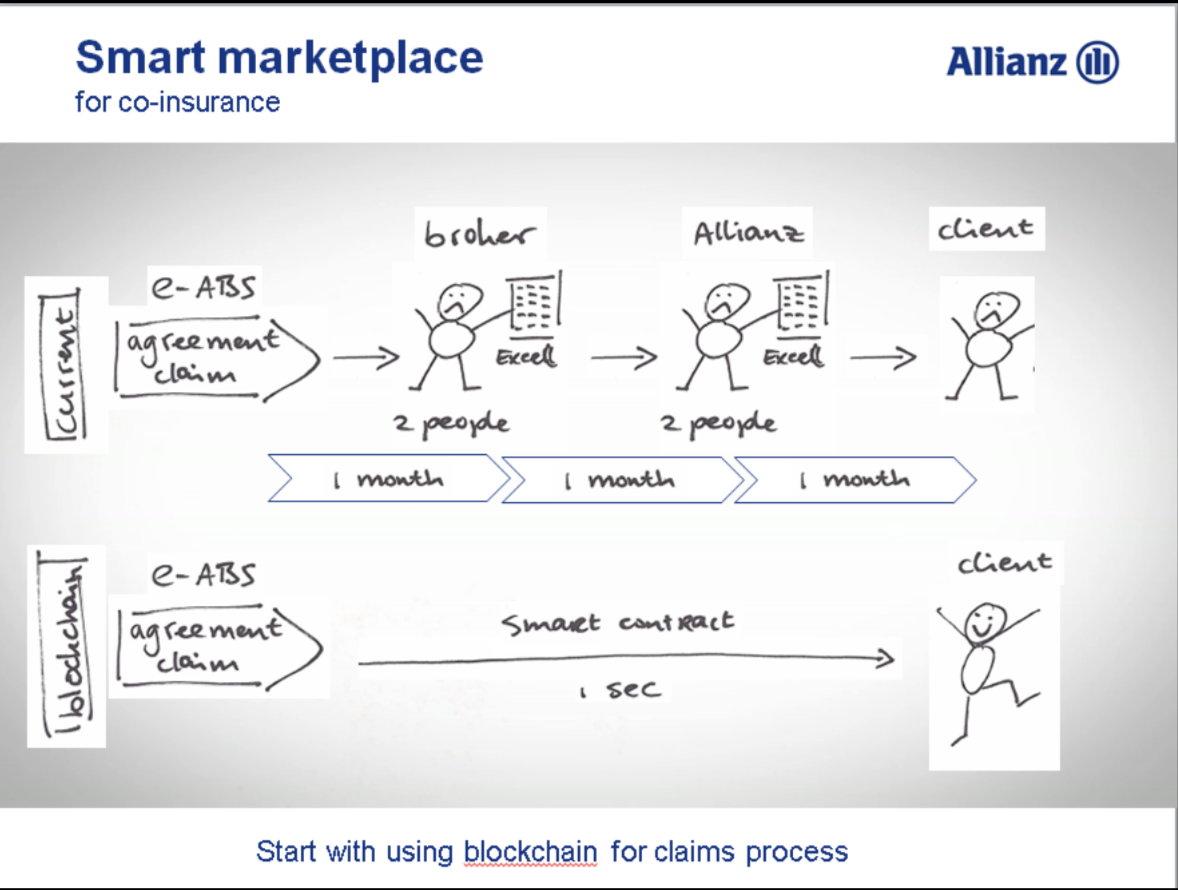
\includegraphics[scale=0.6]{images/allianz-blockchain}
        \caption{Usecase: co-insurance - Allianz}
        \label{fig:allianz-blockchain}
    \end{center}
\end{figure}
